\documentclass[man]{apa6}

% Packages
\usepackage[utf8]{inputenc}
\usepackage[american]{babel}
\usepackage{csquotes}
\usepackage[style=apa,backend=biber]{biblatex}
\usepackage{graphicx}
\DeclareLanguageMapping{american}{american-apa}
\usepackage{comment}

% Load Citations
\addbibresource{citations.bib}

% Self Explanatory

\title{The Effect of Memory Cue Duration on  
Directed Forgetting Performance in Healthy Aging}

\shorttitle{Memory Cue Duration and Directed Forgetting}

\author{Kyle Kurkela, Courtney Allen, Nancy Dennis}

\affiliation{Pennsylvania State University}

\date{\today}

\abstract{Although forgetting is usually seen as a memory error, intentional forgetting can function as an adaptive mechanism to manage information in an ever changing world. XXXXXXXXX. However, many cognitive processes, including directed forgetting, decline with age. Thus, one of the goals of the current investigation was to elucidate a strategy – allowing for increased processing time – that could be employed to enhance memory and executive functioning and to compensate for age-related deficits. The current study employed an item-method directed forgetting paradigm combined with the Remember/Know/New (R/K/N) paradigm to examine the effect of increased memory cue durations (one, three, and five seconds) on directed forgetting in younger (18-30 years) and older (60-85 years) adults. Results indicated that increased processing time improved directed forgetting performance in both age groups. Although no significant age-related deficit in directed forgetting was observed between these two groups, subsequent analyses revealed a significant interaction between older adults’ level of general cognitive functioning and directed forgetting performance. Furthermore, the expected age-related deficit emerged in these analyses, with respect to the lower-functioning older adults. These findings indicate the importance of considering individual differences in cognitive aging research.}

\keywords{directed forgetting, older adults, cue durations, memory}

\authornote{This project was supported by American Federation for Aging Research (AFAR) grant 421-55 2B2G. In addition, my thanks go to Kristina Peterson, former lab manager of the Cognitive Aging and Neuroimaging Lab, undergraduate research assistant Christina Johnson, and former undergraduate research assistants David Hoagey, Matt McGee, and Joanna Zappalla for their assistance with this project.}

% Body of the Document Begins
\begin{document}

% Title Page
\maketitle

% Introduction

In an age where we are besieged with information, often times it is just as important to learn how to forget information, as it is to remember it. While incidental forgetting is ***, intentional or goal-directed forgetting represents ***. The process of intentional forgetting has been studied using the Directed Forgetting (DF) paradigm. In item-method DF, participants are presented with a series of items, each followed by a cue instructing the individual to either remember (often called a to-be-remembered (TBR) cue) or forget the item (often called a to-be-forgotten (TBF) cue). Participants, however, are ultimately asked to attempt to remember all of the stimuli, regardless of the original cue \parencite{bjork1970,bjork1972,bjork.woordward1973,basden1996}. One’s ability to intentionally forget information is typically operationalized as the difference in forgetting for TBF items compared to forgetting for TBR items (termed the DF-effect). 

Two theories have been offered to explain this often observed DF-effect. Originally, the DF-effect was explained by the Selective Rehearsal Hypothesis, which posited that TBR items were better remembered than TBF items because the TBR items were subject to increased processing at encoding \parencite{bjork1970,paller1990,basden.badsen.Gargano1993}. That is, a remember cue led to deeper and more elaborate processing, whereas the presentation of a forget cue essentially halted any further processing. This differential encoding, in turn, led to better memory for TBR items with no effect on the TBF items, which were presumably incidentally encoded. Recently, it has been proposed that while TBR items undergo differential encoding, TBF items are not simply passively dropped from memory, but are actively inhibited from gaining access to long-term memory stores \parencite{fawcett.taylor2008,zachs.hasher1994,zacks.radvansky.hasher1996}. In other words, in addition to the TBR cue boosting subsequent memory through deep encoding, the TBF cue evokes active inhibitory processes that suppress encoding processes. In addition to behavioral evidence, the Attentional Inhibition Hypothesis is well supported by neuroimaging studies that show that, compared to a TBR cue, a TBF cue elicits differential activity in right superior and middle frontal gyri \parencite{ullsperger.mecklinger.muller2000,paz.menor.jimenez2004,wylie.foxe.taylor2008,rizio.dennis2013}, regions associated with other cognitive inhibition processes \parencite{anderson.et.al.2004,depue.curran.banich2007,benoit.anderson2012,anderson.huddleston2012,levy.anderson2012}.

With regard to aging, past research has found a reduced DF effect in older compared to younger adults \parencite{andres.vanderlinden.parmentier2004,collette.et.al.2009,dulaney.marks.link2004,earles.kersten2002,feyereisen.charot2008,gamboz.russo2002,hasher.zacks.rahhal1999,hogge.adam.collette2008,lustig.hasher.zacks2007,sego.golding.gottlob2006} \parencite[see][for meta-analysis and review]{zachs.hasher1994,zacks.radvansky.hasher1996,titz.verhaeghen2010}. Researchers have suggested that age deficits in DF arise from decline in both differential encoding and inhibition mechanisms \parencite{zacks.radvansky.hasher1996, zacks.hasher.li2000, hogge.adam.collette2008}. This conclusion is supported by studies showing that older adults have a more difficult time initiating deep encoding \parencite[for review, see]{craik.rose2012} and inhibiting irrelevant material \parencite[e.g.,]{troyer.leach.strauss2006, lawo.et.al.2012}. The latter finding has formed the basis of the Inhibition Deficit Theory of aging, which attributes age-related cognitive deficits to a decline in inhibitory control of working memory contents \parencite{hasher.zacks1988,zacks.hasher.li2000}. However, central to the design of the DF paradigm are constraints on the timing to execute each cognitive process. That is, participants typically are given only a few seconds to either encode or inhibit the presented item. One the foremost theories of cognitive aging posits that age-related decline in cognitive processing is chiefly due to age-related slowing of mental operations \parencite{salthouse1996}. This Processing Speed Theory of aging posits that older adults exhibit poorer cognitive performance compared to younger adults due, in part, to the fact that the time required by early operations (e.g., processing of the memory cue) reduces the time available for later operations (e.g., execution of deep encoding or inhibition).

Both theories of cognitive aging may account for the aforementioned age differences observed in the DF paradigm. That is, in the typical DF paradigm individuals are presented with the memory cue for a very short duration (e.g., 1 second). By restricting processing time in this manner, older adults may incur difficulty processing the memory cue and fully executing differential encoding and inhibitory control processes necessary to direct memory processing. In addition, while age-related deficits in inhibitory control may reduce older adults’ ability to suppress the encoding of TBF items, this may be exacerbated by the short amount of time provided for the execution of this process. Thus, while these two explanations of age differences in DF are not necessarily incompatible, taken together they suggest that observed DF deficits in older adults may be a result if the collective effect of both age-related deficits in inhibition and processing speed. Thus, allowing older adults longer to bring online both encoding and inhibitory mechanisms may serve to both enhance DF in aging and reduce age deficits.

While the length of cue duration in the DF paradigm has been examined previously, results have been mixed. Specifically, research in young adults has shown that increases in cue duration has led to a reduced DF effect \parencite{lee.lee.tsai2007} others observe no effect of duration \parencite{allen.vokey1998,bancroft.hockley.farquhar2013}. Most relevant to the current study is a study by \textcite[Exp. 2]{dulaney.marks.link2004} which examine cue duration in older adults. Using cue durations of 1500, 3000, and 5000 ms researchers observed a significant DF effect in young adults at the two shorter cue durations, but failed to find a statistically significant DF effect at 5000 ms. They also failed to find a significant DF effect in older adults associated with any cue duration. The lack of DF effect in older adults notwithstanding, the study design included a random intermixing of cue duration that may have precluded the authors’ ability to truly test the effect of cue duration. That is, the unpredictable cue duration may have hindered participants’ ability to utilize the longer processing time effectively and older adult’s ability to XXXX. The current study aims to address this methodological concern by blocking trials by cue duration, thus allowing participants to use this knowledge when executing encoding processes.

The current study also aims to expand our understanding of age-related differences in directed forgetting by examining the effect of cue duration in directed forgetting on recollection and familiarity separately. The majority of directed forgetting studies have used a yes/no recognition paradigm \parencite[but see][]{gardiner.gawlik.richardson1994, rizio.dennis2013,rizio.dennis2014plos}. As such, the memory test collapses across qualitative differences in memory (i.e., recollection and familiarity), which are known to be mediated by distinct subsystems of the MTL \parencite[e.g.,][]{diana.yonelinas.ranganath2007mtl, yonelinas.et.al.2005mtl} and show differential effects in aging, with recollection showing greater age-related decline than familiarity \parencite{parkin.walter1992,jennings.jacoby1993,mantyla1993,java1996,davidson.glisky2002,yonelinas2002recfamreview,bastin.vanderlinden2003,howard.et.al2006}.

The current study aims to isolate not only forgetting effects, but also  
 
Also relevant to the current study was a study performed by \textcite{gardiner.gawlik.richardson1994}, which also observed the effects of cue duration on directed forgetting, but importantly utilized a R/K/N paradigm at retrieval. All of the DF studies discussed thus far have utilized a yes/no retrieval response paradigm, allowing for the observation of a single DF-effect. Gardiner and colleagues’ study is unique and relevant to the present study because their study design allows for the observation of three different DF effects, a DF-effect of recollection (i.e. remember responses), a DF-effect of familiarity (i.e., know responses), as well as a DF-effect of a miss rate, analogous to the classic DF-effect seen in the yes/no retrieval paradigm. As has been mentioned previously, this ability to parse out effects of different memory sub-processes is important in the context of aging. To our knowledge, no study to date has examined the effect of cue duration in combination with a R/K/N paradigm in aging.

% Methods

\section*{Methods}

\subsection*{Participants}

Thirty young adults and 33 older adults participated in the study. Three older adults were excluded from all analyses due to: a failure to use all response options, a high depression score as measured by the Geriatric Depression Scale (see below), and a MATLAB error resulting in a failure to record retrieval data. Young adults were Pennsylvania State University undergraduates between the ages of 18 and 23 years (\textit{M} = 19.13 years, SD = 1.41; 25 females) and received class credit for participating. Older adults were Centre County residents between the ages of 61 and 80 years (\textit{M} = 69.47 years, SD = 5.14; 21 female) and were financially compensated for their participation (see Table 1). All participants provided informed consent for the ethical treatment of human participants, approved by the Pennsylvania State University Institutional Review Board.

\subsection*{Materials}

Stimuli consisted of 364 words obtained from the MRC Psycholinguistic Database \parencite{coltheart1981}. The stimuli had a mean \textcite[]{kuvcera.nelson1967} written frequency of 108.65 (SD = 56.41), and a mean word concreteness \parencite{spreen.schulz1966,gilhooly.logie1980} of 420.49 (SD = 101.73). Two hundred and forty words were used during encoding, separated equally into 3 duration conditions (1000, 3000, and 5000 ms). The remaining 120 words were used as foils during the recognition test. All words were presented in the center of the computer screen in uppercase white letters on a black background. Memory cues were also presented centrally on a black background. To-Be-Remembered (TBR) cues consisted of five green pound signs, while To-Be-Forgotten (TBF) cues consisted of five red pound signs. The order of TBR and TBF cues was pseudo-random such that no more than three of each trial-type were ever presented in a row. Equal numbers of TBR and TBF cues were presented in each cue duration condition. The remaining 4 words were used to practice the task prior to the encoding phase.

\subsection*{Procedure}

\subsubsection*{Cognitive Assessment}

Prior to participation in the experimental protocol, all participants completed a battery of neuropsychological tests including: the Mini-Mental State Examination \parencite{folstein.robins.helzer1983mmse}; sections of the Wechsler Adult Intelligence Scale (WAIS-III) and Wechsler Memory Scale (WMS-III), including Symbol Search, Digit-Symbol Coding, Symbol Copy, Digit Span, Arithmetic, Letter-Number Sequencing, and Vocabulary \parencite{wais2008}; and either the Beck Depression Inventory (BDI-II) \parencite{beck.et.al.1996bdi}, or the Geriatric Depression Scale (GDS) \parencite{yesavage.sheikh1986gds}. Raw scores for the Symbol Search, Digit-Symbol Coding, Digit Span, Arithmetic, Letter-Number Sequencing, and Vocabulary tasks were standardized based on age at time of test. To measure overall cognitive functioning, all standardized scores were averaged to obtain a single measure of baseline cognitive ability.

\subsubsection*{Encoding}

In the encoding task, participants were presented with a series of words, displayed one-at-a-time on the computer screen for 1000 ms (see Figure 1). Each word was followed by a brief 2000 ms delay, during which a white fixation cross was presented. To ensure that participants were attending to stimulus presentation, participants were further instructed to indicate whether or not each word contained the letter ‘A’. After this period, a memory cue was presented in the center of the screen indicating whether the word was to-be-remembered or to-be-forgotten. Cues consisted of a group of five colored pound signs. Participants were instructed that words followed by green pound signs should be remembered (TBR items), as they would appear on an upcoming memory test, whereas words followed by red pound signs should be forgotten (TBF items), as they would not be on the memory test. A 2000 ms inter-trial interval preceded the next item, during which a blue fixation cross appeared on the screen. Trials were further broken down into 3 blocks corresponding to cue duration [1 sec (1000 ms), 3 sec (3000 ms), or 5 sec (5000 ms)]. See Figure 1 for design parameters. Each encoding block contained 80 items: 40 TBR and 40 TBF words, resulting in total of 120 TBR and 120 TBF words presented during encoding. The presentation order of the 3 encoding blocks was counterbalanced across participants.

\subsubsection*{Retrieval}

Following a 10 min interference task [Arithmetic Test for young adults and Matrix Reasoning for older adults \parencite{wais2008}], participants completed a retrieval task for the words they had previously studied (see Figure 2). The interference task was followed by a retrieval task that included 360 words: 120 TBR targets, 120 TBF targets, and 120 novel lures. Each word appeared individually on the screen for 2500 ms during which time participants were asked to make a remember/know/new (R/K/N) memory decision \parencite[see][for a review]{yonelinas.jacoby1995remknow}. It was stressed to the participants that their memory response should not depend on whether the word had been associated with a TBR or TBF cue during encoding but should instead depend only on whether the word was old or new. The retrieval task was divided into 5 runs of 72 words each.

\section*{Results}

\subsection*{DF Effect Calculations}

Prior to performing statistical analyses, two different directed forgetting effects were calculated for each age group for each condition: the Traditional Directed Forgetting Effect and a Recollection Effect. The Traditional DF Effect was operationalized, in accordance with previous DF studies (citations), as the proportion of TBF targets receiving a new response minus the proportion of TBR targets receiving a new response (i.e., TBF-Forget –TBR-Forget). This measure served as an indicator of directed inhibition performance. Because the current study used a R/K/N retrieval paradigm, we were also able to calculate a Recollection Effect, which was operationalized as the proportion of TBR targets receiving a recollection response minus the proportion of TBF targets receiving a recollection response and served as our indicator of directed remembering performance \parencite{rizio.dennis2014plos}.

As mentioned in the Introduction, the current study had an a-priori hypotheses about Recollection/Remembering and Forgetting/Inhibition in aging and thus the above two memory effects serve as the basis of the current analyses. The use of the R/K/N paradigm, however, also allows us to calculate another remembering effect, the Familiarity Effect. Specifically, we calculated an independent measure of familiarity operationalized as the proportion of targets that did not receive a remember response that received a familiarity response \parencite{yonelinas.jacoby1995remknow,jacoby.yonelinas.jennings1997} (see supplemental materials). This independent familiarity effect was subjected to the same analyses as the Recollection Effect, the results of which are reported in supplemental materials.

\subsection*{Replication}

Prior to performing analyses on our variables of interest (i.e., Cue Duration, Age Group, and Cognitive Ability), we wanted to determine if we had successfully replicated the previously reported Traditional DF and Recollection Effects in our sample of younger and older adults collapsed across our Cue Duration conditions. One sample t-tests of the Traditional DF and Recollection Effects revealed that both our younger and older adult samples displayed, collapsed across Cue Durations, mean Traditional DF and Recollection Effects that were significantly greater than zero (both \textit{p}s < .001). Additional one-sample t-tests were also run to determine if our memory effects of interest were significantly greater than zero within each Cue Duration within each Age Group. Our sample of young and older adults both displayed Traditional DF Effects that were significantly greater than zero in the 3 and 5 second Cue Duration conditions (all \textit{p}s < .001), but did not show significant Traditional DF effects in the 1 second cue duration condition (both \textit{p}s = ns, after Bonferroni correction).The Recollection Effects in our two Age Group samples were significantly greater than zero in all three Cue Durations conditions (all \textit{p}s < .01, Bonferroni corrected).

\subsection*{Effects of Cue Duration and Age Group}

\subsubsection*{Traditional Directed Forgetting Effect}

To examine the influence of Cue Duration on the Traditional DF Effects displayed by our young and older adult samples, a 3 (Cue Duration) by 2 (Age Group) repeated measures ANOVA was performed. The ANOVA revealed a significant main effect of Cue Duration (\textit{F}(2,116) = 22.35, \textit{p} < .001). The main effect of Age Group (\textit{F}(1,58) = .340, \textit{p} = ns) and Age Group x Cue Duration (\textit{F}(2,116) = .953, \textit{p} = ns) interaction failed to reach significance. The main effect of Cue Duration manifested itself as an increase in the size of the Directed Forgetting Effect (collapsed across YAs and OAs) from the 1 second cue duration (\textit{M} = .061, \textit{SEM} = .020) to the 3 second cue duration (\textit{M} = .149, \textit{SEM} =.020) to the 5 second cue duration (\textit{M} = .180, \textit{SEM} =.022). Follow up Bonferroni corrected pairwise comparisons revealed that, collapsed across YAs and OAs, the mean Traditional DF Effect in 1 second cue duration condition was significantly smaller than the means in both the 3 second cue duration (\textit{p} < .001) and the 5 second cue duration (\textit{p} < .001) conditions. The means and standard errors of the Traditional DF Effect for YAs and OAs at each Cue Duration are displayed in Figure 3.

\subsubsection*{Recollection Effect}

To examine the influence of Cue Duration on the Recollection Effect displayed by our young and older adult samples, another 3 (Cue Duration) by 2 (Age Group) repeated measures ANOVA was performed. This ANOVA also revealed a significant main effect of Cue Duration (\textit{F}(2,116)=4.96, \textit{p} <. 01). The main effect of Age Group (\textit{F}(1,58) = .020, \textit{p} = ns) and the Age Group x Cue Duration (\textit{F}(2,116) = .058, \textit{p} = ns) interaction failed to reach significance. The main effect of Cue Duration manifested itself as an increase in the Recollection Effect, collapsed across YAs and OAs, from the 1 second cue duration (\textit{M} = .074, \textit{SEM} = .017) condition to the 3 second cue duration (\textit{M} = .100, \textit{SEM} = .015) condition to the 5 second cue duration (\textit{M} = .127, \textit{SEM} = .016) condition. Follow up Bonferroni corrected pairwise comparisons revealed that, collapsed across YAs and OAs, the mean effect size in the 1 second cue duration was significantly smaller than the mean effect size in the 5 second cue duration (\textit{p} < .05, corrected). The means and standard errors of the Recollection Effect for YAs and OAs at each Cue Duration are displayed in Figure 3.

In order to further clarify the foregoing ANOVA results, we performed follow up analyses aimed at clarifying the effect of Cue Duration within each Age Group. We tested all of the pairwise comparisons between the levels of cue duration within each age group (previous pairwise comparisons reported above were collapsed across age group) for both of our memory effects. The results of these Bonferroni corrected pairwise comparisons revealed the following. Our older adult sample displayed increasing mean Traditional DF Effects, with the 1 second cue duration condition being significantly smaller than the 3 second cue duration (\textit{p} < .01) and significantly smaller than the 5 second cue duration (\textit{p} < .001). Younger Adults displayed the same pattern of mean effect sizes for the Traditional DF Effect, with the mean effect size in the 1 second cue duration being significantly smaller than the 3 second cue duration (\textit{p} < .001) and significantly smaller than the 5 second cue duration (\textit{p} < .001; See Figure 3). None of the Bonferroni corrected pairwise comparisons for the Recollection Effect reach significance for either age group (all \textit{p}s > .05, corrected). 

\subsection*{Individual Differences in Cognitive Baseline}

In order to test our \textit{a-prori} hypothesis that only highly cognitively able participants’ will be able to take advantage of increases in cue duration, we ran 12 linear regressions (one for each cue duration, for each effect, for each Age Group) to test the statistical significance of the linear relationship between Baseline Cognitive Assessment Score and mean effect size in each cue duration condition. Bonferroni corrected for multiple statistical tests, the regressions revealed a single statistically significant regression of cognitive measures predicting the traditional DF effect in the 5 second cue duration for Older Adults (\textit{R}$^{2}$ = .362, \textit{F}(1,27) = 15.31, \textit{p} < .001, $\beta$ = .053; see Figure 5). To further clarify the difference in the relationship between Cue Duration and Cognitive Ability, we ran pairwise t-tests on the regression slopes (i.e., $\beta$s) of the 3 cue durations for the Traditional DF effect in OAs. The results of the pairwise one tailed t-tests between these 3 beta values revealed that the regression slope in the 5 second cue duration was significantly greater than in the 3-second cue duration (\textit{t}(27) = 1.99, \textit{p} < .05) and the 1-second cue duration condition (\textit{t}(27) = 22.25, \textit{p} < .05). The difference between the 1 and 3 second cue duration did not reach significance (\textit{t}(27) = -0.17, \textit{p} > .05). As a last follow-up, we ran a one tailed t-test, testing statistical significance of difference in regression slopes between the Traditional DF Effect, OA, 5-second Cue Duration regression and the YA Traditional DF Effect, YA, 5-second Cue Duration regression. The results of this t-test suggests that the difference in the slopes is not statistically different (\textit{t}(54) = .07, \textit{p} = ns). 

\section*{Discussion}

The current study has four major conclusions. First, increased processing time can benefit differential encoding processes for both younger and older adults, which will be discussed in the context of \textcite{salthouse1996}'s Processing Speed Theory of age-related cognitive deficits. Second, while young adults were able to enhance inhibition with increased processing time, older adults displayed no significant differences in inhibition among any of the cue durations. The finding that older adults are unable to reap an inhibitory benefit with increased processing time implicates an inherent inability for older adults to improve intentional forgetting, which will be considered with respect to \textcite{hasher.zacks1988}' inhibition deficit theory of cognitive aging. Third, our analyses indicated the absence of an age-related deficit in the DF-effect at all cue durations when considering recollection, familiarity, and an analogue to the traditional effect. Due to this unusual result, the lack of an age difference was further explored through a follow up analysis which sought to test the hypothesis that increases in processing time would help OAs inhibition performance for those OAs with higher baseline cognitive ability. Results indicated that the higher-functioning OAs showed significantly better directed forgetting performance, and that the level of cognitive functioning was a significant predictor of inhibition performance only when OAs were given 5 seconds to processes the cue. This finding demonstrates the importance of considering individual variability in cognitive aging research \parencite{nelson.dannefer1992, christensen.et.al1994, morse1993,shammi.bosman.stuss1998,  christensen.et.al1999, anstey.christensen2000,  christensen2001}. Finally, analyses indicated that lower-functioning older adults were unable to utilize longer cue durations to improve their directed remembering effect. However, higher-functioning older adults were able to utilize additional time to improve both differential encoding and inhibition. These results contribute to the discussion of the importance of considering individual differences and variability in cognitive aging research. These conclusions are further elaborated below. 

\subsection*{Increased Cue Duration and Differential Encoding in Young and Older Adults}

Young adults showed significant DR-Effect improvement between the one-second and three-second memory cue durations, as well as between the one-second and the five-second durations. These results suggest that the increased processing time generally improves young adults’ differential encoding processes. However, this improvement in differential encoding leveled off after the three-second duration, with no memory benefit conveyed with the increased increment of time from three to five seconds. Therefore, we must consider whether differential encoding success is directly related to processing time for young adults. In other words, it may not be possible for young adults to continuously improve differential encoding performance with increased processing time; rather, they may reach a ceiling past which they cannot improve (see Figure 3). 

Similar to young adults, older adults’ directed forgetting performance benefited from increased memory cue durations; however, their differential encoding processes garnered a significant benefit at every interval of increased cue duration. Their DR-Effect values significantly increased from one to three seconds, one to five seconds, and three to five seconds (see Figure 3). 

Young and older adults’ differing patterns of differential encoding enhancement with increased processing time indicate a relationship between processing speed and task-specific cognitive demands. \textcite{salthouse1996} posited that an inevitable reduction in processing speed is the fundamental deficit underlying age-related cognitive decline. Logically, this reduction in processing speed impairs performance by preventing task completion under limited time conditions. As a result, older adults can only access incomplete, partially processed information, a limitation that manifests as cognitive deficits in a variety of tasks. This idea formed the basis of the current investigation: if older adults directed forgetting performance shows an age-related decline because they are unable to complete differential encoding and inhibitory processes within the given task framework, providing more processing time within the task should allow for more complete execution of these processes. Older adults’ continual improvement in differential encoding across all cue conditions corroborates this reasoning. At each duration, their performance improved because they were able to more fully execute differential encoding processes. Therefore, older adults’ DR-Effects should continue to improve until an optimal cue duration is reached, at which point differential encoding processes are being executed completely. It may be possible that this optimal duration is not five seconds, and that older adults’ differential encoding would continue to improve with even longer cue durations. 

On the other hand, young adults’ DR-Effect values level off at three seconds. This ceiling may occur because young adults are able to fully execute differential encoding processes within three seconds, having not yet experienced age-related decline in processing speed. Therefore, further increasing processing time to five seconds or more would likely confer no additional enhancement to young adults’ already completed differential encoding processes.

\subsection*{Increased Cue Duration and Inhibition in Young and Older Adults}

Although increased processing time improved differential encoding for both young and older adults, only young adults’ showed significant improvement in inhibition as a result of the memory cue duration manipulation. The increased processing time between one and five seconds conferred a significant benefit only to young adults’ inhibition mechanisms. In addition, no ceiling was apparent in regards to the F-Effect; therefore, it is possible that young adults’ inhibitory mechanisms could further benefit from processing time exceeding five seconds. 

Thus, it seems that inhibitory processes operate within a different time frame than those of differential encoding. While differential encoding seems to be a finite cognitive process that is completed within three seconds for young adults, inhibition seems to be an ongoing process of suppression. As a result of the increased time duration from one to five seconds, young adults were able to forget more TBF items, suggesting that these items became less accessible in working memory as the duration of inhibition increased. Consistent with this interpretation, these data suggest that the longer information is suppressed in memory, the less accessible it becomes. 

Contrastingly, older adult data indicated no significant differences between F-Effect values at any of the cue durations. These results – in which differential encoding, but not inhibition, improves as a result of increased processing time – are consistent with the conclusion that differential encoding and inhibition processes differ in their characteristics and in the cognitive demands they incur. With respect to the Processing Speed Theory of cognitive aging \parencite{salthouse1996}, older adults’ inhibitory processes should have improved with increasing cue duration, if inhibition was indeed impaired due to the fact that it lacked sufficient processing time to complete. The absence of this improvement supports the idea that there is more at play in older adults’ directed forgetting performance than processing speed impairments, and that inhibition is not a finite cognitive process. 

Rather, our results suggest that older adults’ inhibitory processes seem to be fundamentally impaired, such that increased processing time cannot benefit task performance. Such an interpretation is consistent with \textcite{hasher.zacks1988}' inhibition deficit theory of cognitive aging, which states that older adults’ have a fundamental deficit in inhibition. In the current study, older adults’ inhibition was preserved enough to exhibit the directed forgetting effect. However, consistent with the inhibition deficit framework, they were unable to enhance inhibitory processing past this baseline level due to the inherent age-related decline in inhibition. 

\subsection*{Older Adults’ Individual Variability Contributes to the Lack of an Age-Related Decline}

Although age-related cognitive deficits are well documented, no significant age-related differences in directed forgetting performance were observed in the current investigation. This absence of an age-related deficit in directed forgetting performance is not unheard of in the literature: researchers such as \textcite{gamboz.russo2002} also did not observe the expected age-related directed forgetting deficit. The fact that not all older adult populations exhibit age-related deficits indicates variability between different populations of older adults. In order to explore how individual differences within our population of older adults may have resulted in the absence of an age-related directed forgetting deficit, median split analyses were conducted based on level of cognitive functioning, as defined by cognitive assessment performance. 

Previous research indicates that variability is greater in older adults than in other populations. \textcite{nelson.dannefer1992} analyzed 127 gerontological studies, concluding that diversity increases with age across a wide variety of domains. Similarly, \textcite{morse1993} analyzed existing literature comparing young and older adult variability, finding that variability increased with age across domains of reaction time, memory, and fluid intelligence. Consistent with these findings, median split analyses conducted in the current investigation revealed large significant differences in directed forgetting performance between higher- and lower-functioning older adults, but no differences between higher- and lower-functioning young adults. 

Moreover, the highly disparate performance of higher- and lower-functioning older adults is consistent with research reporting a great deal of individual variability within populations of older adults. For example, \textcite{shammi.bosman.stuss1998} reported high levels of inter-individual variability among older adult participants on cognitive and psychomotor tasks. In addition, Christensen and colleagues \parencite{christensen.et.al1994,christensen.et.al1999,christensen2001} consistently report greater age-related variability in domains of memory, fluid intelligence, and speed in both cross-sectional and longitudinal studies. 

Therefore, it is well established that individual differences in aging are pervasive factors in the preservation or deterioration of cognitive functioning. As such, it is necessary to consider their contribution to task performance, in order to provide a more meaningful picture of cognitive aging than is provided through mean-level analyses \parencite{nelson.dannefer1992}. Surprisingly, the current study is among the first investigations reflecting upon the contribution of age-related individual variability in cognitive functioning on directed forgetting performance. In order to gain a comprehensive understanding of cognitive aging, similar analyses of individual differences should become an integral step in the reporting process of cognitive aging research. 

\subsection*{Variability in Cognitive Functioning Predicted Utilization of Increased Cue Duration}

Further analyses were conducted to determine if level of cognitive functioning influenced older adults’ ability to enhance directed forgetting performance with increased processing time. Higher-functioning older adults significantly improved both differential encoding and inhibition from one to five seconds, and from three to five seconds. However, lower-functioning older adults showed no significant interaction amongst any of the cue durations for either differential encoding or inhibition. Overall, these results suggest that higher-functioning older adults were able to use increased processing time to improve directed forgetting, while lower-functioning older adults could not utilize increased cue duration to their beneficial at all. This lack of benefit is unexpected because, in the overall older adult analyses, significant improvement in differential encoding was evident between each memory cue duration condition. Therefore, higher-functioning older adults’ directed forgetting performance elevated the lower-functioning group’s scores such that the overall older adult averages misleadingly indicated a significant benefit of increased processing time, which did not exist for lower-functioning older adults. 

Furthermore, the median split analyses clarified the lack of an age-related directed forgetting deficit. As in the previous instance, the higher-functioning older adults’ directed forgetting performance elevated the lower-functioning group’s values so that there appeared to be no age-related decline in directed forgetting, when lower-functioning individuals did in fact display this expected deficit. Therefore, it seems that cognitive functioning is predictive of performance in directed forgetting, and perhaps in other cognitive tasks. However, it is unknown how cognitive functioning has this impact, and what factors contribute to variability in this area. 

Previous research has attempted to identify predictors underlying older adults’ variability in cognitive task performance. One of the most prevalent predictors of cognitive performance is degree of education, such that more years of education confers a protective advantage to older adults’ cognition \parencite{christensen.et.al1999,anstey.christensen2000,christensen2001}. Indeed, the current investigation revealed a positive correlation between degree of education and level of cognitive functioning. Thus, perhaps degree of education is either a factor impacting, or a reflection of, cognitive functioning. 

Previous research has also suggested that variability in speed and reaction time may underlie cognitive deficits, particularly for women \parencite{morse1993,christensen.et.al1999,christensen2001}. Therefore, \textcite{salthouse1996}'s Processing Speed Theory of age-related cognitive decline still validly predicts the results of the current study, given the added consideration that the degree of older adults’ processing speed impairment varies based on the individual. The potential for greater variability amongst females is also interesting, since the current study’s older adult sample was predominantly female. In conclusion, individual differences are important factors to consider in age-related cognitive decline, and definitively characterizing predictors of cognitive functioning in old age is an important area for future research. 

\section*{Conclusion}

Overall, the current study demonstrates that increased processing time within an item-method directed forgetting task improves directed forgetting performance in both young and older adults. Specifically, young adults’ differential encoding improved from one second to three seconds, and their inhibitory processes improved from one second to five seconds. Older adults, on the other hand, showed enhancement only in differential encoding, but displayed a more consistent pattern of improvement than young adults, benefiting from increased time at each increased cue duration. These results were considered with respect to both \textcite{salthouse1996}'s Processing Speed Theory of age-related cognitive decline and \textcite{hasher.zacks1988} inhibition deficit theory of cognitive aging. However, analyses did not indicate an age-related deficit. 

In order to better characterize the absence of an age-related directed forgetting deficit, we performed median split analyses based on level of cognitive functioning. Results indicated that, at five seconds, lower-functioning older adults displayed significantly worse directed forgetting performance than higher-functioning older adults. In addition, the lower-functioning group exhibited the expected age-related directed forgetting deficit. Finally, only higher-functioning older adults were able to utilize increased cue durations to improve directed forgetting performance. Therefore, lower-functioning older adults that displayed the typical age-related directed forgetting deficit were not able to use increased processing time to compensate for age-related directed forgetting deficits. While increased processing time appeared to be an effective strategy to improve directed forgetting performance in young and higher-functioning older adults, it did not benefit the lower-functioning group most in need of enhancement. 

Finally, the current investigation has broader implications for the field of cognitive aging in general. The current study and many other researchers question the utility of theories of cognitive aging that seek to identify a single cause for age-related decline. It is better to consider the combination of age-related deficits, task-specific characteristics, and individual differences \parencite{albinet.et.al2012}. The current study investigated the impact of individual differences in cognitive functioning on directed forgetting performance, revealing significant differences between higher- and lower-functioning older adults. Characterizing individual differences is an important future direction in cognitive aging research, especially since individual variability is greater among older adults than in other populations. 

\printbibliography

% Tables

% Figures
\begin{figure}
    \centering
    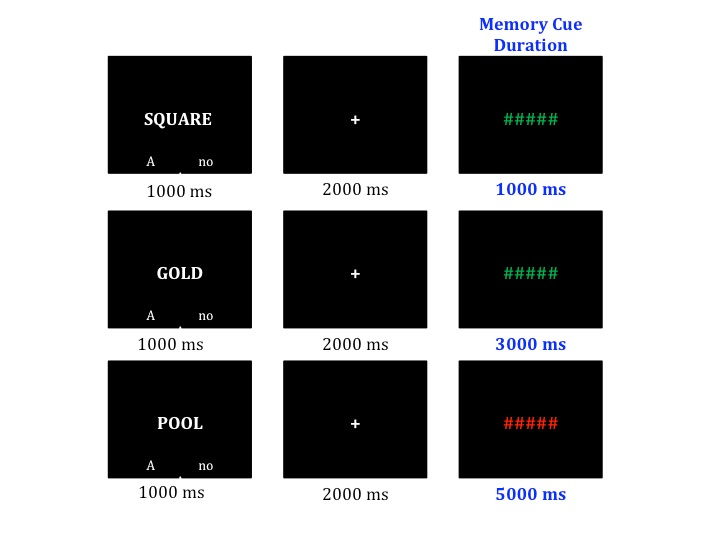
\includegraphics[width=\textwidth]{Slide1.jpg}
    \caption{A visual summary of the item-method directed forgetting encoding task for each memory cue duration. Participants completed a shallow encoding task for each word (Does the word contain the letter 'A' or not?). Subsequently, each word was followed by a memory cue instructing participants to either remember (green) or forget (red) the previous word.}
    \label{fig:1}
\end{figure}

\begin{figure}
    \centering
    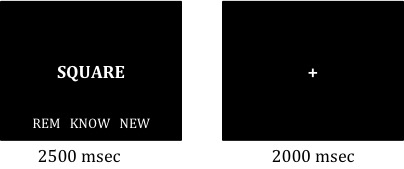
\includegraphics{Fig2.jpg}
    \caption{A visual summary of the item-method directed forgetting retrieval task (Remember/Know/New) for all words from encoding (120 TBR, 120 TBF) and 120 new items. Participants had 2.5 seconds to indicate their memory response to the word.}
    \label{fig:2}
\end{figure}

\appendix

\section{Appendix A}

\subsubsection{Independent Familiarity Effect}

In investigating effects on familiarity, it is important to note that recollection and familiarity are not necessarily mutually exclusive mechanisms of memory functioning. As such, the raw proportion of ‘Know’ responses to targets does not provide an independent measure of familiarity because it is inherently dependent on a participants use of the remember response \parencite[see][]{jacoby.yonelinas.jennings1997,yonelinas.jacoby1995remknow}. In other words, increase use of the remember response necessitates a decreased in the use of the know response and vice-versa. To account for this interdependence between response options, we used a  measure of familiarity where familiarity rates were defined as the proportion of targets not given a ‘Remember’ response that are given a ‘Know’ response \parencite{yonelinas.jacoby1995remknow}(e.g., Jonathan M Fawcett, Lawrence,  Taylor, 2016; Andrew P Yonelinas  Jacoby, 1995). The independent familiarity estimates were then used to calculate a second directed remembering effect, a Familiarity Effect, by subtracting the estimate of familiarity for TBR items from that of the TBF items.

Like with the remembering effect, we first wanted to determine if our sample of YAs and OAs displayed a Familiarity Effect that was significantly greater than zero. To do so, we performed a one-sample t-test on the mean Familiarity Effect for YAs and OAs collapsed across Cue Durations.The tests confirmed our hypotheses, suggesting that the mean effect of YAs and OAs were overall significantly greater than zero (all \textit{t}s(29) > 3.63, \textit{p}s < .01). After this confirmation, we next wanted to confirm that YAs and OAs displayed Familiarity Effects that were significantly greater than zero in each of the three cue durations conditions. One-sample t-tests showed that the mean Familiarity effect was significantly greater than zero in the 3 and 5 second cue duration for both Age Groups (\textit{t}s(29) > 2.93, \textit{p}s < .01), but not in the 1 sec cue duration (\textit{t}s(29) < 1.76, \textit{p}s = ns).

After confirming greater than zero mean effect sizes, we submitted the observed Familiarity Effects to a 3 (Cue Duration) by 2 (Age Group) ANOVA. The results of this ANOVA revealed a significant main effect of Cue Duration (\textit{F}(2, 116) = 13.54, \textit{p} < .001), a main effect of Age Group that failed to reach significance (\textit{F}(1, 58) = .140, \textit{p} = ns), as well as an interaction effect of Cue Duration and Age Group that failed to reach significance (\textit{F}(2, 116) = 2.483, \textit{p} = ns). The main effect of Cue Duration manifested itself as increasing mean effect sizes from the 1 second cue duration (\textit{M} = .036, \textit{SEM} = .021) to the 3 second cue duration (\textit{M} = .118, \textit{SEM} = .021) to the 5 second cue duration (\textit{M} = .143, \textit{SEM} = .021). Follow up Bonferroni corrected pairwise comparisons revealed that the mean effect in the 1 second cue duration condition was significantly less than the means of both the 3 second cue duration condition (\textit{p} < .01) and the 5 second cue duration condition (\textit{p} < .001).

To test our \textit{a-prori} hypotheses concerning the relationship between cognitive ability and increased processing time in directed forgetting, we ran a series of 6 linear regressions using Cognitive Assessment Score to predict the mean Familiarity Effect size in each of the 3 cue duration conditions for both Age Groups. Results revealed a single significant (after Bonferroni correction) regression of Cognitive Assessment Scores predicting the mean Familiarity Effect for OAs in the 5-second cue duration condition (\textit{R}$^{2}$ = .387, \textit{F}(1, 27) = 17.04, p < .001, $\beta$ = .053).

\end{document}
